 \chapter{原子核物理}\label{ch:b3:nuclear-physics}

% Provenance (not for print): first half of the "physique subatomique"
% module common to the surveyed third-year curricula; particle physics
% follows in the next chapter. Deepens the high-school volume's
% radioactivity with SEMF, Gamow tunnelling and reactor physics.

高中分册已勾勒出这一故事的梗概：原子有原子核；
有些原子核会衰变，其时间尺度从微秒
到数十亿年不等；一克物质中竟藏着兆吨级的能量。本章
将用本科三年级的工具重新审视原子核。含五项的液滴模型
能把数百种\omterm{def:b3:nuclear-physics:nuclide}{核素}的结合能预测到
百分之一的精度；隧道效应——即本科二年级分册的势垒问题，经提升后——
解释了一个公式如何跨越
二十五个数量级的 $\alpha$ 衰变寿命；而结合能曲线的
铁处那个平缓的极大值，把全部核技术分成两大阵营：
裂变重核（反应堆）或聚变轻核（恒星，以及
未来的发电厂）。本章结束于反应堆水池旁，
池水闪耀着切伦科夫蓝光。

\section{原子核：饱和液滴}

\begin{definition}[核素、大小与密度]\label{def:b3:nuclear-physics:nuclide}
\index{核素}\index{同位素}\index{核半径}
称 $^{A}_{Z}\text{X}$ 为\emph{核素}，它含 $Z$ 个质子与 $N = A -
Z$ 个中子，二者由\emph{强相互作用}束缚：强度
（接触时约为库仑力的 ${\sim}\qty{100}{}\times$ 倍），短程
（${\sim}\qty{1}{fm}$，仅在相邻核子接触时才能感受到），且
对电荷不敏感（质子与中子被同等地束缚）。散射
实验给出各原子核相同的规律：半径
\[
R = r_0A^{1/3} , \qquad r_0 \approx \qty{1.2}{fm} ,
\]
因此体积正比于 $A$，密度为普适常数
$\rho \approx \qty{2.3e17}{kg/m^3}$——一滴这种物质
重量堪比一支油轮船队，而
在\cref{ch:b3:astrophysics}中，将遇到以此密度存在的整颗恒星。
\emph{同位素}具有相同的 $Z$，而 $N$ 不同：化学性质相同，
但原子核的命运各不相同。
\end{definition}

\begin{proposition}[质量亏损与结合能]\label{prop:b3:nuclear-physics:binding}
\index{质量亏损}\index{结合能}\index{铁峰}
束缚态原子核的质量比其组成部分\emph{更小}；
由\cref{ch:b3:relativistic-dynamics}可知，所缺的质量即为
结合能，
\[
B = \big(Zm_{\text{p}} + Nm_{\text{n}} - m_{\text{原子核}}\big)c^2 ,
\]
通常约为 ${\sim}\qty{8}{MeV}$，\emph{每核子}——相当于
化学能的一百万倍。按每核子绘制，$B/A$ 在轻核区急剧攀升，
（表面效应渐弱），在铁-56 附近达到 $\approx\qty{8.8}{MeV}$ 的峰值，
随后因库仑斥力（长程且不饱和）而缓缓下降，
压制重核。两侧斜坡都是能量宝库：
\emph{聚变}攀上左坡（太阳的工作），
\emph{裂变}沿右坡滚落（反应堆的工作）——而铁，
位于峰顶，对两者而言都是核“灰烬”。
\end{proposition}

\begin{omfigure}
\begin{tikzpicture}
  \begin{axis}[omaxis, axis x line=bottom, axis y line=left,
    width=11.2cm, height=6.2cm, xmin=0, xmax=250, ymin=0, ymax=10.3,
    xlabel={质量数 $A$}, ylabel={$B/A$ (\unit{MeV})},
    xlabel style={at={(axis description cs:0.5,-0.1)}, anchor=north},
    xtick={56,100,150,200,238}, ytick={2,4,6,8}, clip=false]
    \addplot[omDef, very thick, smooth] coordinates {
      (2,1.11) (3,2.7) (6,5.3) (9,6.46) (12,7.68) (16,7.98)
      (24,8.26) (40,8.55) (56,8.79) (75,8.7) (100,8.6)
      (125,8.45) (150,8.3) (175,8.1) (200,7.9) (220,7.75) (238,7.57)};
    \fill[omThm] (axis cs:4,7.07) circle (1.6pt);
    \draw[gray, thin] (axis cs:12.5,6.85) -- (axis cs:5.2,7.02);
    \node[omThm, font=\scriptsize, anchor=west] at (axis cs:13,6.8)
      {$^4$He};
    \fill[omThm] (axis cs:56,8.79) circle (1.6pt);
    \node[omThm, font=\scriptsize, anchor=south] at (axis cs:56,9.0)
      {$^{56}$Fe：峰顶};
    \fill[omThm] (axis cs:238,7.57) circle (1.6pt);
    \node[omThm, font=\scriptsize, anchor=south west] at (axis cs:225,7.85)
      {$^{238}$U};
    \draw[->, omExo, thick] (axis cs:14,4.0) -- (axis cs:40,6.4);
    \node[omExo, font=\scriptsize, anchor=west] at (axis cs:18,3.6)
      {聚变攀升};
    \draw[->, omExo, thick] (axis cs:225,6.4) -- (axis cs:130,7.6);
    \node[omExo, font=\scriptsize, anchor=east] at (axis cs:242,5.9)
      {裂变下行};
  \end{axis}
\end{tikzpicture}

{\small 结合能曲线——堪称物理学中最具影响力的
图像之一。轻核通过合并获益，重核通过分裂获益；
按每千克计，左坡的收益约为右坡的四倍，
而太阳正处在左坡上。}
\end{omfigure}

\begin{proposition}[半经验质量公式]\label{prop:b3:nuclear-physics:semf}
\index{半经验质量公式}\index{稳定谷}
将原子核视为带电液滴，整条曲线
可由五项导出：
\[
B = a_{\text{V}}A - a_{\text{S}}A^{2/3}
- a_{\text{C}}\frac{Z^2}{A^{1/3}}
- a_{\text{A}}\frac{(A - 2Z)^2}{A} + \delta(A) ,
\]
其中（单位 \unit{MeV}）：$a_{\text{V}} = 15.8$（每个核子与其
近邻成键，即体积项），$a_{\text{S}} = 17.8$（表面核子成键
较少，即液滴的“表面张力”），$a_{\text{C}} = 0.71$
（库仑项：长程的破坏者），$a_{\text{A}} = 23.7$
（不对称项：由\cref{ch:b3:quantum-statistics}可知，质子与
中子分别填入两个独立的费米阶梯，两者填充程度相当时代价最小），
而 $\delta$ 为偶数核的小配对项，
（见\cref{ch:b3:identical-particles}）。固定 $A$ 时求极小，描出
\emph{\omterm{prop:b3:nuclear-physics:semf}{稳定谷}}：轻核中 $N \approx Z$，
随库仑力压制质子，曲线向富中子一侧弯折（$N/Z \to 1.5$），
——偏离谷底的\omterm{def:b3:nuclear-physics:nuclide}{核素}则通过 $\beta$ 衰变回到谷中。
\end{proposition}
\admitted

\begin{omfigure}
\begin{tikzpicture}
  \begin{axis}[omaxis, axis x line=bottom, axis y line=left,
    width=8.6cm, height=6.4cm, xmin=0, xmax=95, ymin=0, ymax=150,
    xlabel={质子数 $Z$}, ylabel={中子数 $N$},
    xlabel style={at={(axis description cs:0.5,-0.1)}, anchor=north},
    xtick={20,40,60,80}, ytick={50,100,150}, clip=true]
    \addplot[gray, dashed, domain=0:95] {x};
    \addplot[omDef, very thick, domain=1:92, samples=100]
      {x + 0.03*x^(5/3)};
    \node[gray, font=\scriptsize, anchor=north west] at
      (axis cs:78,74) {$N = Z$};
    \node[omDef, font=\scriptsize, anchor=north west, align=left] at
      (axis cs:48,125) {稳定谷};
    \fill (axis cs:26,30) circle (1.5pt);
    \node[font=\scriptsize, anchor=north west] at (axis cs:26,29) {Fe};
    \fill (axis cs:92,146) circle (1.5pt);
    \node[font=\scriptsize, anchor=north west] at (axis cs:88,143) {U};
  \end{axis}
\end{tikzpicture}

{\small \omterm{prop:b3:nuclear-physics:semf}{稳定谷}示意。轻核平衡其两条
费米阶梯（$N = Z$）；重核则以多余的中子
稀释其库仑代价。偏离谷底的\omterm{def:b3:nuclear-physics:nuclide}{核素}经 $\beta$ 衰变
回到谷中——而远高于该线产生的裂变碎片，
正因如此而极具放射性。}
\end{omfigure}

\section{放射性：按钟计时}

\begin{theorem}[衰变定律]\label{thm:b3:nuclear-physics:decay}
\index{放射性衰变定律}\index{半衰期}\index{放射性活度}
不稳定原子核没有记忆，也不会老化：在其存活的每一秒内，
它以相同的概率 $\lambda$ 衰变。对于 $N$
个原子核，$\dd N = -\lambda N\,\dd t$，于是
\[
N(t) = N_0\,\eu^{-\lambda t} = N_0\,2^{-t/T_{1/2}} ,
\qquad T_{1/2} = \frac{\ln2}{\lambda} ,
\]
而\emph{放射性活度} $\mathcal A = \lambda N$（每秒衰变数，
\unit{Bq}）同样按指数规律衰减。半衰期
从微秒到数十亿年不等。
由\cref{ch:b3:microcanonical-ensemble}中的统计规律可知，单个
原子核完全不可预测，而一摩尔的原子核
所呈现的指数式时间比任何钟都准确——这正是
放射性测年的基础。
\end{theorem}

\begin{proof}
每秒衰变概率恒定，意味着 $N(t + \dd t) = N(t)(1 -
\lambda\dd t)$；积分即得。令 $N/N_0 = \tfrac12$，可得
$T_{1/2}$。
\end{proof}

\begin{omfigure}
\begin{tikzpicture}
  \begin{axis}[omaxis, axis x line=bottom, axis y line=left,
    width=9.8cm, height=5.6cm, xmin=0, xmax=4.3, ymin=0, ymax=1.12,
    xlabel={$t/T_{1/2}$}, ylabel={$N/N_0$},
    xlabel style={at={(axis description cs:0.5,-0.1)}, anchor=north},
    xtick={1,2,3,4}, ytick={0.25,0.5,1},
    yticklabels={$\tfrac14$,$\tfrac12$,$1$}, clip=true]
    \addplot[omDef, very thick, domain=0:4.3, samples=150]
      {exp(-0.6931*x)};
    \draw[gray, dashed] (axis cs:0,0.5) -| (axis cs:1,0);
    \draw[gray, dashed] (axis cs:0,0.25) -| (axis cs:2,0);
    \node[font=\scriptsize, anchor=south west, align=left] at
      (axis cs:2.3,0.55) {每过一个半衰期 \\计数减半};
  \end{axis}
\end{tikzpicture}

{\small 指数衰减：个体无记忆，群体却守时。两个
半衰期后剩四分之一，十个半衰期后则剩千分之一——
这把尺子使物理学家得以测定木炭、
冰川与地球的年龄。}
\end{omfigure}

\begin{remark}[原子核的三条出路]\label{rem:b3:nuclear-physics:modes}
\index{α 衰变}\index{β 衰变}\index{γ 辐射}\index{伽莫夫模型}
$\boldsymbol\alpha$：重核放出一个 $^4$He 团簇。经典意义上
不可能——库仑势垒高达 \qty{25}{MeV}，而
$\alpha$ 粒子逸出时能量仅 \qty{5}{}--\qty{9}{MeV}——它借
\emph{隧道效应}实现（本科二年级分册中的势垒，曲线形）：伽莫夫的
指数式的敏感性使能量相差两倍，
便使寿命相差二十个数量级，正是盖革–纳托尔
规律（见\cref{exo:b3:nuclear-physics:8}）。
$\boldsymbol\beta$：中子变为质子（或反之），放出
一个电子（或正电子）和一个中微子——即\emph{弱相互作用}
在起作用，即让\omterm{def:b3:nuclear-physics:nuclide}{核素}回归谷底的力；中微子的
故事留待\cref{ch:b3:particle-physics}再讲。
$\boldsymbol\gamma$：受激原子核放出 \unit{MeV} 光子，
即原子核中与\cref{ch:b3:hydrogen-atom}中谱线相对应的现象。
衰变一直串联，直至到达谷底：铀的阶梯
经过十四级台阶后，止于稳定的铅。
\end{remark}

\section{下坡之路：裂变与聚变}

\begin{proposition}[裂变与链式反应]\label{prop:b3:nuclear-physics:fission}
\index{裂变}\index{链式反应}\index{临界质量}
慢中子被 $^{235}$U 吸收后，形成一个振荡的液滴，
随即分裂：产生两个中等质量的碎片、两到三个新中子，以及
$\approx\qty{200}{MeV}$——即铀与碎片的 $B/A$ 之差：
铀为 \qty{7.6}{MeV}，碎片为 \qty{8.5}{MeV}，乘以 235。
释放出的中子可引发其他原子核裂变：
设倍增因子为 $k$（每代中子数之比），
则中子数按 $k^n$ 增长——次临界（$k < 1$）
逐渐消亡，临界（$k = 1$）维持稳定，超临界则爆发式增长。
反应堆借慢化剂将中子减速（裂变最偏好的“食粮”），
并依赖那 0.7\,\% 的中子，它们因碎片衰变而
\emph{迟到数秒}——正是这一延迟使 $k \approx 1$ 可由人调节，
并使控制棒得以吸收过剩的中子
（见\cref{pb:b3:nuclear-physics:1}）。
\end{proposition}
\admitted

\begin{omfigure}
\begin{tikzpicture}[scale=1.0]
  % stage 1: nucleus + neutron
  \draw[->, thick] (-1.3,0) -- (-0.55,0);
  \fill[gray] (-1.55,0) circle (2.6pt);
  \node[font=\scriptsize, anchor=south] at (-1.55,0.12) {中子};
  \draw[omDef, fill=omDef!15, thick] (0.35,0) circle (0.62);
  \node[omDef, font=\scriptsize] at (0.35,0) {$^{235}$U};
  % arrow
  \draw[->, thick] (1.35,0) -- (2.05,0);
  % stage 2: deformed drop (peanut)
  \draw[omDef, fill=omDef!15, thick, rotate around={0:(3.1,0)}]
    (3.1,0) ellipse (0.85 and 0.42);
  \draw[omDef!60, dashed] (3.1,-0.5) -- (3.1,0.5);
  % arrow
  \draw[->, thick] (4.3,0) -- (5.0,0);
  % stage 3: fragments + neutrons
  \draw[omThm, fill=omThm!12, thick] (5.9,0.55) circle (0.42);
  \draw[omThm, fill=omThm!12, thick] (5.9,-0.55) circle (0.42);
  \node[omThm, font=\tiny] at (5.9,0.55) {Ba};
  \node[omThm, font=\tiny] at (5.9,-0.55) {Kr};
  \foreach \ang in {15,-8,40}{
    \fill[gray] ({6.7+0.35*cos(\ang)},{0.3*sin(\ang)}) circle (2.2pt);
    \draw[->, gray] ({6.95+0.35*cos(\ang)},{0.32*sin(\ang)}) --
      ({7.55+0.35*cos(\ang)},{0.42*sin(\ang)});}
  \node[font=\scriptsize, anchor=west, align=left] at (8.05,0)
    {2--3 个中子 \\$+\ \qty{200}{MeV}$};
\end{tikzpicture}

{\small 液滴模型裂变：慢中子使 $^{235}$U 发生振动；形变液滴中的
库仑斥力压倒了表面张力，于是它撕裂成富中子的碎片
与多余的中子，
正是这些中子使链式反应成为可能。}
\end{omfigure}

\begin{remark}[聚变：更难、但更好的斜坡]\label{rem:b3:nuclear-physics:fusion}
\index{聚变}
轻核聚合时，每千克释放的能量约为
重核裂变的 $\sim4\times$ 倍，且没有长寿命的碎片——但
参与反应的两个原子核都带正电，必须穿越彼此之间的
库仑势垒，这要求温度达到 $10^7$--$10^8\,\unit{K}$
（见\cref{exo:b3:nuclear-physics:11}）。恒星靠体积庞大来实现这一过程
（见\cref{ch:b3:astrophysics}：太阳每秒将 \qty{600}{} 百万吨氢转化为氦）；
实验室则借助磁约束的等离子体来实现，
而迄今为止，其能量收支仍
远未达到收支平衡的目标。
\end{remark}

\begin{omfigure}
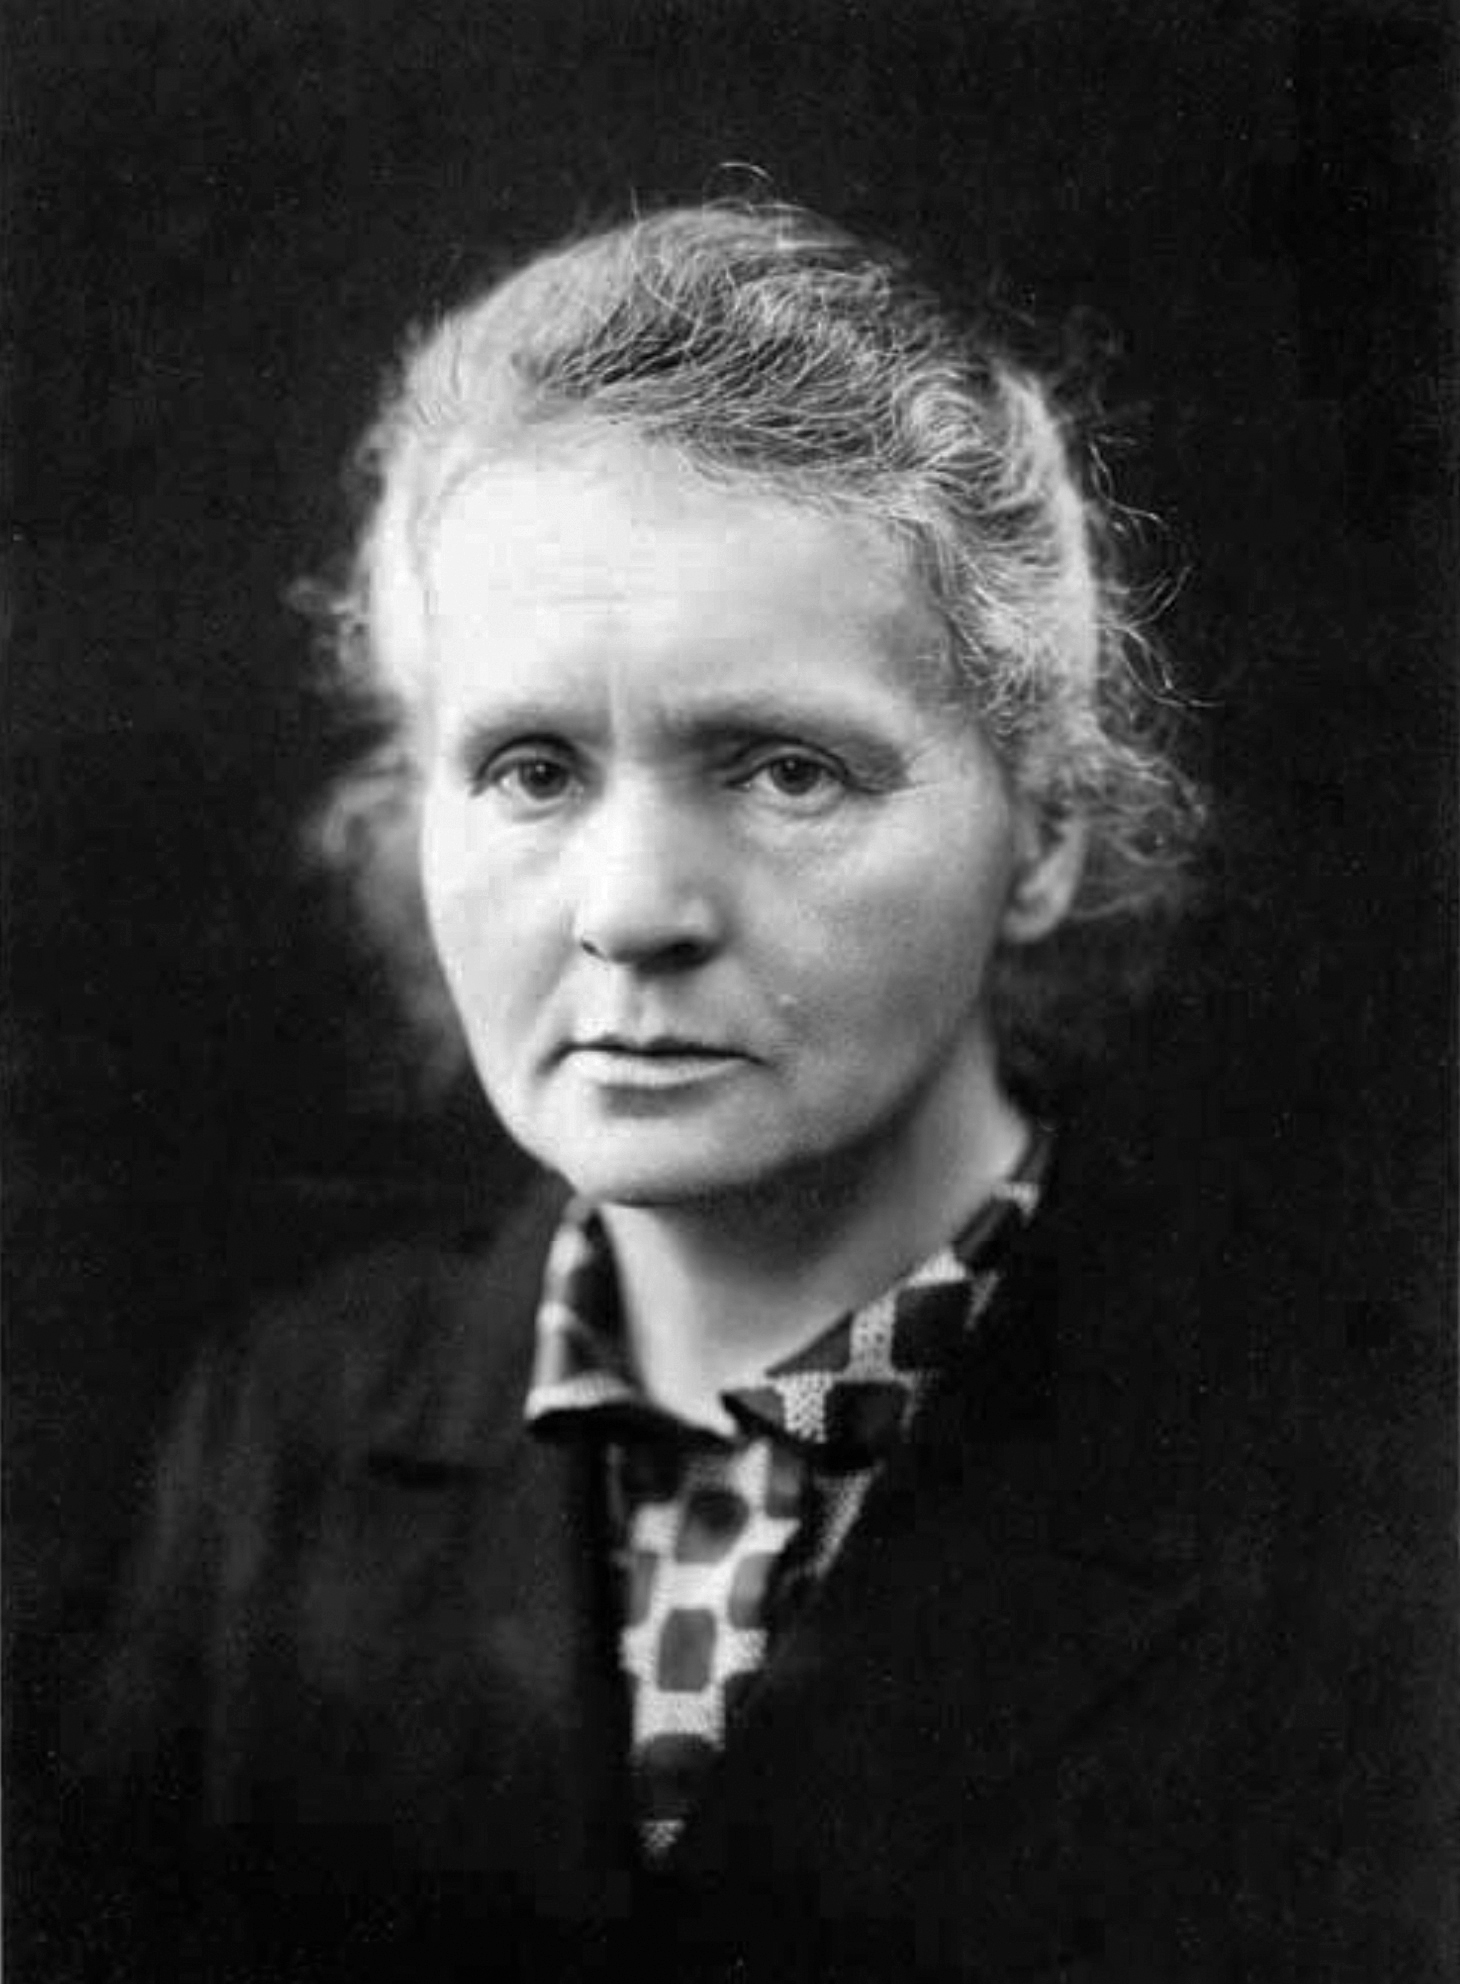
\includegraphics[width=0.34\linewidth]{images/book5/photo-marie-curie.jpg}

{\small 玛丽·居里（照片：Henri Manuel，约 1920 年，公有领域）：因开创本章的研究主题两度获得诺贝尔奖；\cref{exo:b3:nuclear-physics:4} 中的那一克镭正是属于她的。}
\end{omfigure}

\section{练习}

\begin{exercise}[$\star$]\label{exo:b3:nuclear-physics:1}
\omterm{def:b3:nuclear-physics:nuclide}{核素}统计。(a) 求 $Z$、$N$、$A$：$^{12}$C、$^{14}$C、
$^{235}$U、$^{238}$U。(b) 哪些是\omterm{def:b3:nuclear-physics:nuclide}{同位素}？(c) 为什么\omterm{def:b3:nuclear-physics:nuclide}{同位素}化学性质相同，
而核稳定性却不同？(d) $^{14}$C 与 $^{14}$N 的 $A = 14$ 相同：
这类\omterm{def:b3:nuclear-physics:nuclide}{核素}称为什么，
它们之间通过何种衰变相联系？
\end{exercise}

\begin{exercise}[$\star$]\label{exo:b3:nuclear-physics:2}
普适的密度。(a) 由 $R = r_0A^{1/3}$，证明原子核的密度
与 $A$ 无关，并求其值。(b)
计算一茶匙（\qty{5}{mL}）核物质的质量。
(c) 原子核占原子体积的几分之几（取
$R_{\text{原子}} = \qty{1e-10}{m}$，$A = 60$）？(d)
$A^{1/3}$ 律本身对强相互作用的作用范围说明了什么？
\end{exercise}

\begin{exercise}[$\star$]\label{exo:b3:nuclear-physics:3}
称量“胶水”。核质量：$m_{\text{p}} =
\qty{1.007276}{u}$，$m_{\text{n}} = \qty{1.008665}{u}$，
$m(^4\text{He}) = \qty{4.001506}{u}$；
$\qty{1}{u}\,c^2 = \qty{931.5}{MeV}$。(a) 求 $^4$He 的\omterm{thm:b3:relativistic-dynamics:emc2}{质量亏损}
与结合能。(b) 求 $B/A$。(c)
将 $B$ 与 \cref{ch:b3:hydrogen-atom} 中的 \qty{13.6}{eV} 相比较：
核“胶水”与原子“胶水”相差几个数量级？(d) 为什么
$^4$He 异常高的结合能（图中的尖峰）使它
成为 $\alpha$ 衰变中的“通货”？
\end{exercise}

\begin{exercise}[$\star$]\label{exo:b3:nuclear-physics:4}
第一个居里。镭-226：$T_{1/2} = 1600$ 年，摩尔质量
\qty{226}{g/mol}。对于一克镭：(a) 数出原子核的数目；(b) 求 $\lambda$；
(c) 求放射性活度，并与历史上的单位
$1\,\text{Ci} = \qty{3.7e10}{Bq}$（按定义恰好等于这一克镭的
活度）相比较；(d) 经过 4800 年后，这一克镭还剩多少？
\end{exercise}

\begin{exercise}[$\star\star$]\label{exo:b3:nuclear-physics:5}
公式的应用。取 $a_{\text{V}} = 15.75$，
$a_{\text{S}} = 17.8$，$a_{\text{C}} = 0.711$，
$a_{\text{A}} = 23.7$（\unit{MeV}），偶-偶核的对能项
$+12/\sqrt A$：(a) 求四个主要项。
$B$ 对 $^{56}$Fe（$Z = 26$）的各项。(b) 求和（计入对能），并将
$B/A$ 与实测值 \qty{8.79}{MeV} 相比较。(c) 哪两项
相互竞争最激烈？它们的平衡决定了什么？(d) 为什么
为什么库仑项单独的增长必须\emph{快于} $A$？
\end{exercise}

\begin{exercise}[$\star\star$]\label{exo:b3:nuclear-physics:6}
谷底的位置。(a) 只保留与 $Z$ 有关的项，
在 $A$ 固定时使质量最小化，并推导出
$Z^* = \dfrac{A/2}{1 + a_{\text{C}}A^{2/3}/4a_{\text{A}}}$。(b)
对 $A = 101$ 求值，并与钌（$Z = 44$）比较。
(c) 证明轻 $A$ 极限下 $Z^* = A/2$，并借助两个
费米阶梯加以解释。(d) 一个裂变碎片的 $A = 95$，
$Z = 36$：它偏离谷底多远？接下来将经历怎样的
衰变序列？
\end{exercise}

\begin{exercise}[$\star\star$]\label{exo:b3:nuclear-physics:7}
放射性碳定年。活体物质持续补充 $^{14}$C
（$T_{1/2} = 5730$ 年）补充，使其比例保持为每 $10^{12}$
个碳原子中含 1 个；死亡后补充即停止。(a) 一块木炭样品显示
活体活度的 30\,\%，问这堆火距今多少年？(b) 一克活体碳，计算其
$^{14}$C 活度（
预期约为 $\approx\qty{0.23}{Bq}$）。(c) 为何此法在超过
$\sim\qty{50000}{}$ 年后失效？(d) 为何它也无法用于
测定岩石年代（应由哪种“时钟”接替）？
\end{exercise}

\begin{exercise}[$\star\star$]\label{exo:b3:nuclear-physics:8}
伽莫夫悬崖。钋-212 发射一个 \qty{8.78}{MeV} 的 $\alpha$ 粒子；
其势垒顶约为 $\approx\qty{26}{MeV}$。(a) 证明经典逃逸
是不可能的，经典意义下的进入同样不可能——然而它却在
\qty{0.3}{\micro s} 内衰变。(b) 铀-238 的 $\alpha$ 粒子能量为
\qty{4.2}{MeV}，其半衰期为 $4.5\times10^9$ 年：
计算两者的衰变常数之比。(c) 借助隧道效应的指数因子，说明
能量提高一倍，便换来速率
$\sim10^{24}$ 倍的增长。(d) 同样的物理
为何也决定了太阳核心的温度要求？
\end{exercise}

\begin{exercise}[$\star\star$]\label{exo:b3:nuclear-physics:9}
两亿电子伏特。(a) 论证每次裂变释放
$\qty{200}{MeV}$ 的能量（由 $B/A$ 曲线得出）。(b) 计算一千克 $^{235}$U
完全裂变所释放的能量，分别以焦耳和
吨油当量（
\qty{42}{GJ/t}）表示。(c) 一座效率为 33\,\% 的 \qty{1}{GW_e} 发电站，
每年需消耗多少千克 $^{235}$U？(d) 为何是碎片，而非中子，
携带了大部分的
\qty{200}{MeV}，它立即转化为何种形式？
\end{exercise}

\begin{exercise}[$\star\star\star$]\label{exo:b3:nuclear-physics:10}
驯服 $k$。在反应堆中，瞬发中子的繁殖时间为 $\ell
\approx \qty{e-4}{s}$。(a) 若仅考虑瞬发中子，取 $k = 1.001$，
计算一秒内的功率放大倍数，并说明对机械控制的结论。
(b) 若中子中占比 $\beta =
0.7\,\%$ 的中子被\emph{延迟}，延迟约 $\sim\qty{10}{s}$，
解释为何当 $k - 1 < \beta$ 时，链式反应的有效时钟
变为秒量级。(c) 以相同方式计算一秒内的
功率放大倍数，取有效代际时间 $\sim\qty{0.1}{s}$。(d) 用一句话说明
切尔诺贝利操作人员在反应堆转为瞬发超临界时
丧失了什么。
\end{exercise}

\begin{exercise}[$\star\star\star$]\label{exo:b3:nuclear-physics:11}
太阳的算术。总体而言，$4\,^1\text{H} \to {}^4\text{He}$
将 \qty{0.71}{\percent} 的质量转化为能量
（包括中微子在内，\qty{26.7}{MeV}）。(a) 由 $L_\odot =
\qty{3.8e26}{W}$，计算每秒转化的质量，以及每秒消耗的
氢。(b) 取太阳质量为 $\qty{2e30}{kg}$，其中
十分之一为可燃的核心氢（取氢的质量分数
$\approx0.75$）：估算其寿命。(c) 两个质子处于
\qty{1.5e7}{K} 下，比较 $k_{\text{B}}T$ 与它们的库仑
势垒（\qty{1}{fm} 处）的高度，并判断由谁来完成
穿越（见\cref{exo:b3:nuclear-physics:8}）。(d) 与裂变不同，聚变为何
几乎不留下放射性“灰烬”？
\end{exercise}

\begin{exercise}[$\star\star\star$]\label{exo:b3:nuclear-physics:12}
核医学。(a) 锝-99m（$T_{1/2} = \qty{6}{h}$，
$\gamma$ 射线能量为 \qty{140}{keV}）是医学的主力：计算
注入 \qty{500}{MBq} 活度所对应的原子核数目及其质量。
(b) 解释为何\emph{六小时}的半衰期与纯 $\gamma$ 辐射，
各自恰好是诊断所需要的。(c) PET：来自 $^{18}$F 的正电子
与一个电子湮灭——借助\cref{ch:b3:relativistic-dynamics}，
给出两光子的能量与
几何分布，并由此说明探测器的原理。
(d) 放射治疗向肿瘤输送 \qty{2}{Gy}（\unit{J/kg}）的剂量，
将其能量与一小口温水相比较，并调和
焦耳的无害性与电离的致死性。
\end{exercise}

\begin{omfigure}
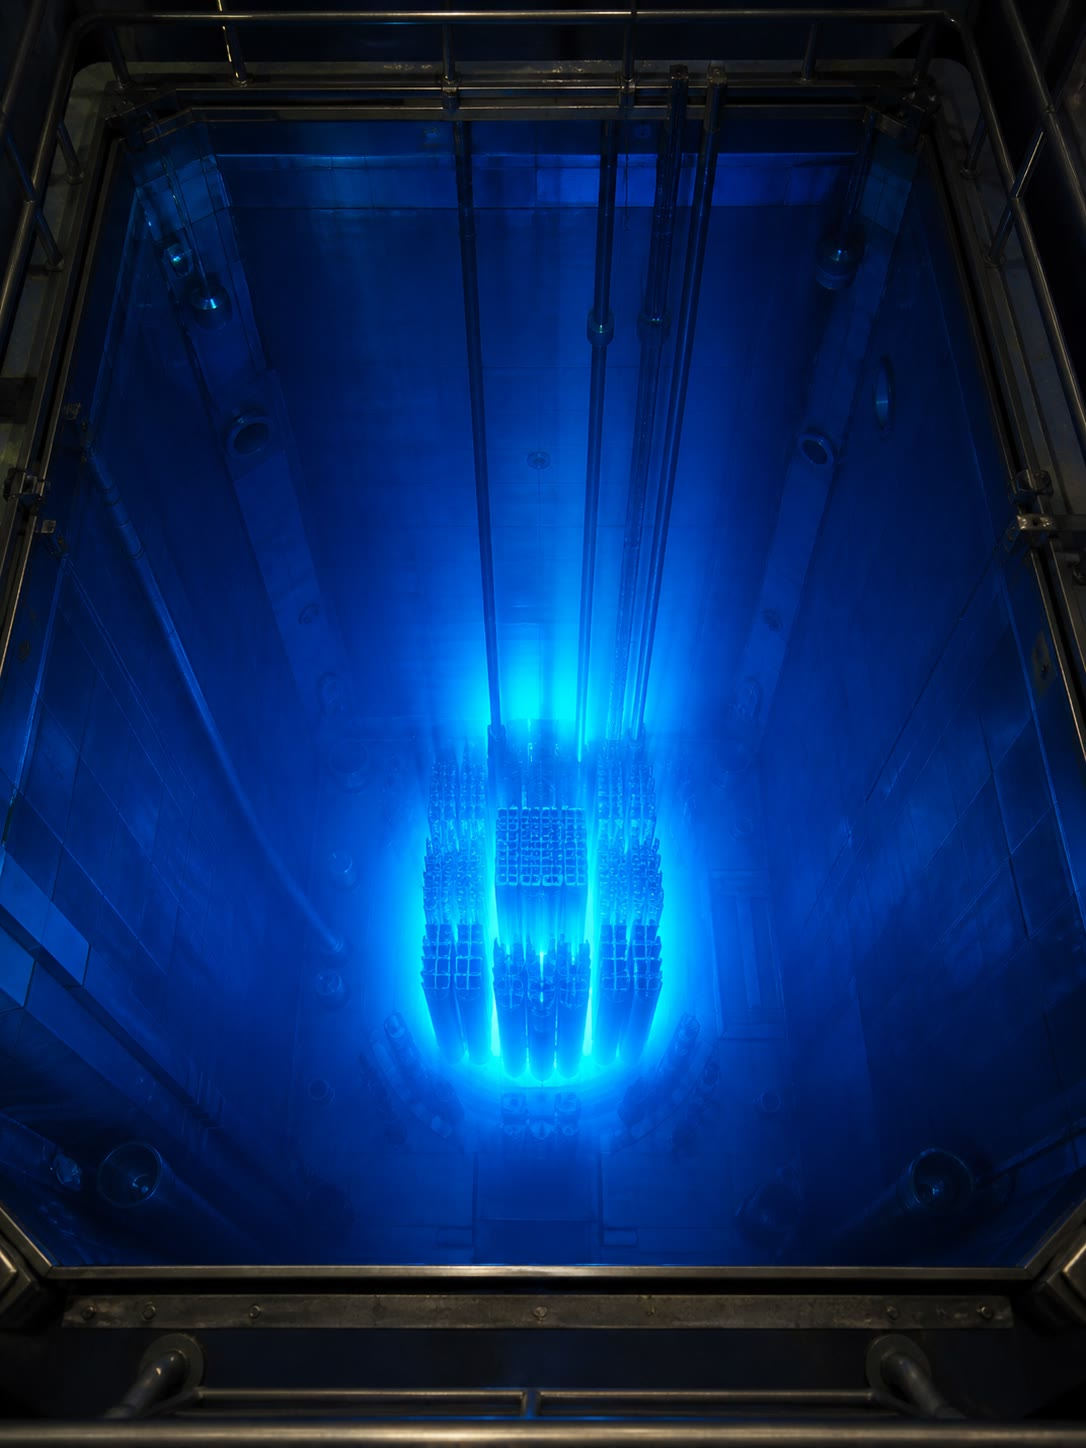
\includegraphics[width=0.45\linewidth]{images/book5/ai/b5-21-cherenkov-pool.jpg}

{\small 周末问题中的反应堆水池：裂变碎片发出的 $\beta$ 电子速度超过水中光速，使堆芯笼罩在切伦科夫蓝光之中——屏蔽作用清晰可见。}
\end{omfigure}

\section{问题：研究用反应堆的开放日}

\begin{problem}\label{pb:b3:nuclear-physics:1}
\emph{研究用反应堆开放日。}国家实验室
向参观者开放其 \qty{20}{MW} 池式研究用反应堆，而你已
设法登上阳台：下方透过八
米清澈的水，堆芯发出一种不似尘世的蓝光。讲解员——
一位即将退休的反应堆物理学家——已同意
让你亲自算一算。

\medskip\noindent\textbf{第一部分 --- 能量账目。}

\begin{enumerate}
  \item 每次 $^{235}$U 裂变约释放 \qty{200}{MeV}。
        将其换算为焦耳，并计算维持
        \qty{20}{MW} 功率所需的每秒裂变次数。
  \item 换算为每日消耗的 $^{235}$U 克数。
  \item 同样的 \qty{20}{MW} 由煤（\qty{30}{MJ/kg}）提供：每天需
        要多少吨？计算两者的质量比，并将其与
        本章的\unit{MeV}与\unit{eV}尺度，以及
        化学中的尺度相联系。
  \item 碎片出生时每个核子的结合能约为 $\sim\qty{8.5}{MeV}$，
        铀则为 \qty{7.6}{MeV}，验证
        $235\times0.9 \approx \qty{200}{MeV}$ 是相容的。
  \item 碎片在距其产生处数微米之内停止。
        它们的 \qty{200}{MeV} 转化为何种形式，并
        以何种时间尺度传至冷却水中？
  \item 为何碎片（例如 $A = 95$，$Z = 36$）
        必然具有放射性？请借助\omterm{prop:b3:nuclear-physics:semf}{稳定谷}加以说明。
\end{enumerate}

\medskip\noindent\textbf{第二部分 --- 保持 $k = 1$。}

\begin{enumerate}[resume]
  \item 定义增殖因子 $k$，并说明
        $k = 0.999$、$1.000$、$1.001$ 分别对
        中子群体意味着什么。
  \item 水池中的水起慢化作用。用两句话说明
        将中子减速到热速率，为何能\emph{促进}
        $^{235}$U 的裂变，以及氢为何是最好的慢化剂
        （回顾本科一年级分册中的弹性碰撞）。
  \item 控制棒由硼钢制成。硼起什么作用，并
        升降控制棒如何调节 $k$？
  \item 仅考虑瞬发中子（$\ell = \qty{e-4}{s}$）
        且 $k = 1.0005$，计算一秒内的功率增长，
        并作出结论。
  \item 缓发中子（占 0.7\,\%）的缓发中子使有效
        代时间延长至 $\sim\qty{0.1}{s}$，重新计算，并
        给出能使 $k - 1$ 安全低于
        缓发份额的设计准则。
  \item 水同时也是冷却剂。请说明固有的
        安全特性：若水沸腾蒸干，慢化作用 --- 进而
        $k$ --- 会发生什么变化？
  \item 停堆之后，反应堆为何仍需
        应急冷却？（请指出控制棒
        无法作用的热源。）
\end{enumerate}

\medskip\noindent\textbf{第三部分 --- 蓝光。}

\begin{enumerate}[resume]
  \item 这种辉光是切伦科夫辐射：水中的光速为
        $c/n$，其中 $n = 1.33$。带电粒子必须怎样运动，
        才能发出这种辐射？
  \item 计算阈值速率，并结合
        \cref{ch:b3:relativistic-dynamics}，求出
        电子的阈值动能。
  \item 反应堆中哪些粒子符合条件？请追踪这一链条：
        从裂变碎片到水中快速 $\beta$ 电子。
  \item 光谱强度随波长变短而增大，
        为何水池发出蓝光而非红光？
  \item 指南写道：“辉光\emph{正是}屏蔽
        发挥作用的表现”。解释一下：八米厚的水
        对堆芯辐射有何作用，阳台为何大致
        安全？
  \item 停堆后，蓝光在数分钟内变暗，
        但数日内并不会消失。请联系第一部分第 6 题。
\end{enumerate}

\medskip\noindent\textbf{第四部分 --- 反应堆的用途。}

\begin{enumerate}[resume]
  \item 本反应堆的日常工作是生产钼-99
        （$T_{1/2} = \qty{66}{h}$），是医学中
        锝-99m 的母体。为何全球医院必须每周
        补货一次，为何没有任何仓库能够囤积它？
  \item 一批 \qty{100}{GBq} 的 Mo-99 于星期一发出，
        医院于星期五（96 小时后）淋洗出 Tc-99m。
        此时母体的放射性活度还剩多少？
  \item 来自堆芯的中子束还为
        \cref{ch:b3:crystalline-solids}中的衍射仪器提供束流：
        反应堆中子一经热化，为何恰好
        具有合适的波长？
  \item 指南的最后一题：一根燃料元件在装运前
        需在水池中停留五年。利用碎片的
        半衰期组成，说明其中的道理 --- 五年
        水池停留换来了什么？
  \item 估算停堆一小时后的衰变热
        （约 $\approx1\,\%$ 的 \qty{20}{MW}），并与
        家用电热器比较：被动式水池冷却是否
        可行？
  \item 用四句话收束全部账目：$B/A$ 使每次
        裂变获得 \qty{200}{MeV}；缓发中子提供了
        使 $k$ 可控的秒量级时间；水兼具慢化、
        冷却、屏蔽与发光的作用；而这一天真正的
        产物装在医用小瓶中运出，而非兆瓦。
\end{enumerate}
\end{problem}
